\section{User-Centered Design}
User-Centered Design (UCD) is a method in which the future users are involved from the start\cite{handbook-usability}.
This ensures that the structure, content and design of the end product are largely driven by the needs, expectations and understanding of the user.
Because a product is only a valuable product if it is actually used by the user.
The closer the product is to the goals and wishes of the users, the more attractive it is for them.
There are different approaches to implement these goals and desires.
Mainly, this can be broken down into three iterative phases.
First, a foundation must be established using various research methods.
Based on this basis, a first conceptual design is developed.
These solutions must then be evaluated together with the users.
This evaluation often leads to new problems, which first have to be investigated, solved, designed and re-evaluated.\\

\subsection{Interviews}
These three phases will also be run through as part of the development of UK4You.
In the first research phase, interviews were carried out to gain different perspectives on the platform to be developed.
A market analysis was also carried out, which will be examined in more detail after this section.
In order to identify as many problems as possible, both bachelor's and master's students were surveyed.
Ideally, employees, doctoral students or professors would also be interviewed at this point.
However, there was not an option to do this during the survey period.
The sample size of $n=5$ is also far too small to be able to make statements about everyone at the University of Kassel.
Nevertheless, better statements can be made about the platform than if the sample size would be $n=1$.\\

The interviews were conducted using an interview guideline (see \autoref{sec:guideline}).
Normally, semi-structured interviews would be conducted at this point because they are more exploratory compared to guided interviews. \textcolor{red}{cite?}
This is because questions are asked in order to shed more light on facts or to explore ideas further.
At this point, however, it was deliberately avoided in order to gain personal experience with structured interviews and to experience the advantages and disadvantages of both interview-types.\\

The interviews were recorded with a microphone after the consent of the individual students.
The audio files were then transcribed into literal, non-phonetic, transcripts.
The audio transcription process offers the advantage that individual passages in a text can be referenced more easily.
Recorded data can also be anonymized and pseudonymised in this way.

\subsubsection{Demographic Data}
The questions in the interview initially related to demographic data.
This data should give more information about preferences based on e.g. the age group or the desired degree.
This data could already contain valuable clues that reveal something about the intended platform design.
Two out of three people who are interested in staying in academia also have a profession that has a university connection. \textcolor{red}{transcripts}
This could suggest that, from the student's perspective, the profession offers an opportunity to enhance success in academia.
With such a small sample size, however, it is unfortunately not really possible to talk about a correlation.
This must also be taken into account for all further statements about the data analysis.\\

Based on the available data, however, it can be seen that the students surveyed want to take different paths in life.
More specifically, there is an academic and professional interest here.
It is important that the platform to be developed offers the opportunity to promote both interests in order to make the platform productive.
Another finding is that all participants are fluent in both German and English.
This can give us more insight into the planned language of the platform.
The University of Kassel requires foreign students to be able to speak the German language.
However, all participants also have the ability to speak English.
This means that nothing would speak against a primarily English platform.
This would also further promote the language skills of the users of the platform.
For foreign students, however, this could be the opposite case, because they do not deepen their knowledge of the German language on the platform.
However, the argument that English is used as the world language and that scientific work is also written in this language is more predominant.\\

\subsubsection{Social media}\label{sec:social-media}
After the questions about demographic data, the students were asked about their social media usage behavior.
Criticism of social media was also surveyed.
The first finding was that all users use social media on a daily basis. \textcolor{red}{transcripts}
In a semi-structured interview, you could follow up here to find out what the reasons are or at what times social media is used.
However, as already mentioned, inquiries were deliberately avoided.
This information may indicate that UK4You will also be used on a regular basis.
In order to ensure productivity, care should be taken that users do not stay on the platform for too long and are only presented with relevant information.
Exactly what relevant content is and how it is suggested is explained in more detail later in the report.\\

\begin{figure}[ht]
    \centering
    \begin{tikzpicture}[scale=0.8]
        \pie{12.5/Discord, 12.5/WhatsApp, 18.75/Instagram, 18.75/Facebook, 37.5/Other}
    \end{tikzpicture}
    \caption{Used social media platforms}
    \label{fig:pie-chart-social-media}
\end{figure}

\autoref{fig:pie-chart-social-media} shows the used social media platforms that were identified in the interviews.
It becomes clear that the use of the media is very diverse.
It should be noted here that the students were not strongly guided to recap all social media and may not have listed some.
The definition of social media also seems to be unclear.
The statements \glqq I would argue that Discord is also a social media platform [...]\grqq{} and \glqq [...] WhatsApp if that counts.\grqq{} are strong an indication of this. \textcolor{red}{transcripts}
Various definitions exist, which is why instant messaging services can be partly included as social media and partly excluded.
A paper attempted to summarize these different definitions and four important points were identified\cite{social-media-definition}.
\begin{enumerate}
    \item Social media are Web 2.0 Internet-based applications
    \item User-generated content is the lifeblood of social media
    \item Individuals and groups create user-specific profiles for a site or app designed and maintained by a social media service
    \item Social media services facilitate the development of social networks online by connecting a profile with those of other individuals and/or groups
\end{enumerate}
In this report, instant messaging services are also considered as social media.\\

The Other-category in particular includes two noteworthy platforms.
These two platforms are called Signal and Mastodon\cite{signal}\cite{mastodon}. \textcolor{red}{transcripts}
They are interesting because they are based on values such as privacy and decentralization.
These platforms are also alternatives to existing platforms.
Signal can be seen as a privacy-focused alternative to the popular WhatsApp platform and Mastodon as a decentralized alternative to Twitter.
The other platforms mentioned in the Other-category are ArtStation, YouTube, Twitter and Telegram. \textcolor{red}{transcripts}\\

If you look at the companies behind the mentioned social media, you can see that the company Meta is behind 50\% of the votes.
While only three of the ten platforms used belong to Meta (Facebook, Instagram and WhatsApp), these are also the most used platforms alongside Discord.
This company, like some other social media platforms, has come under criticism.
In 2021, this took on a new dimension when whistleblower Frances Haugen was able to show that Meta was aware of the harmful societal impact of its platforms\cite{whistleblower-meta}.
However, this report is not intended to examine them in detail.
Of course, the points were still taken into account in the later design and are also explained, but no longer explicitly with reference to Meta or other companies.\\

Everyone uses their mobile device to access social media. \textcolor{red}{transcripts}
Three of the five users also use the PC to consume content or write to others. \textcolor{red}{transcripts}
There are various possible reasons why the students surveyed prefer mobile devices.
On the one hand, it could be because it's much more convenient to look at the phone than to boot up the PC.
On the other hand, it could also be due to the fact that the students surveyed also want to consume content outside their own living space.
This can be on a train ride or a walk, for example.
For the UK4You platform design, it can be said that ideally it should be available for both mobile and stationary devices.\\

Another finding is that four out of five users are passive on social media and do not produce their own content.
Unfortunately, it is difficult to draw the conclusion from this finding that mainly passive users can be found on the UK4You platform and only 20\% actively post content.
However, if you add data from other social media, you can see that up to around 80\% of the users of a platform are passive users.
Of course, this varies from platform to platform and could also be completely different for UK4You.
The important lesson to be learned from this is to pay attention to both types of use and not ignore the passive users in the design process.
While these may have the least interaction with the platform, they often make up the largest percentage.\\

There are various reasons why the surveyed students use social media.
In summary, there are three different reasons.
The first reason is gathering information in some form.
This can be inspiration for your own works, discovering new things or general information in the form of news. \textcolor{red}{transcripts}
The second reason is entertainment to kill boredom. \textcolor{red}{transcripts}
The final reason is to keep in touch with people, be they acquaintances, friends or family. \textcolor{red}{transcripts} \\

Audience research company GWI has found similar results\cite{gwi-top-10-reasons}.
42\% of the motivations to use social media is to stay in touch with what friends are doing.
With just one percent less, the next reason is to be up-to-date with news and current events.
3rd place with 39\% and 4th place with 37\% are killing time or consuming entertaining content.\\

The important question is what conclusions can be drawn from these reasons for UK4You.
Important information should be provided for the first reason from the interview.
This could be course content or further education sources at a university.
Satisfying the second reason might prove more difficult because it stands in stark contrast to the value productivity.
Using UK4You as a platform to kill boredom with fun or entertaining content would make users less productive.
They might also be distracted from productivity by the platform if they come across such content by accident.
The last reason points to having a messaging system that makes it possible to exchange a wide variety of content.\\

The last two questions in the area of social media deepen the points already mentioned.
This is done by listing the pros and cons of using social media.
Thanks to these preferences, previous usage behavior can also be better explained.
Users report that they have an increased interest in information being available quickly and easily. \textcolor{red}{transcripts}
This also goes hand in hand with the usage behavior from before, that users prefer their mobile devices because they offer easier access.
It seems important to one person that the focus is on the content and not on the people themselves.\textcolor{red}{transcripts}\\

UK4You should also be a platform that is strongly content-oriented and less self-promotional or similar.\textcolor{red}{transcripts}
Profiles should be highly customizable, but the whole thing should be kept in moderation.\textcolor{red}{transcripts}
This would also mean that the platform remains productive and is mainly intended for generating, sharing or consuming knowledge.\textcolor{red}{transcripts}
This flow of information should also be up-to-date and not disturbed by marginal information.\textcolor{red}{transcripts}
How this can look like will be shown later in the design proposal.
The possibility of anonymity was also addressed.\textcolor{red}{transcripts}
This could be guaranteed by pseudonyms.
However, there are good reasons against pseudonymization on the UK4You platform.
\autoref{sec:vsd} explains this topic and others based on specific values in detail.\\

However, there are also negative criticisms of social media, which were mentioned in the interviews.
Along with the flow of information mentioned above, one possible consequence would be that there would be a flood of information that would make the platform too overloaded.\textcolor{red}{transcripts}
This information overload could be made worse by advertising on the platform.\textcolor{red}{transcripts}
It is also important to mention that false information can also be spread destructively or unknowingly.\textcolor{red}{transcripts}
One possible way to overcome the information overload is to only suggest relevant content and prevent users from navigating through the platform uncontrolled.
However, it is difficult to define relevant content.
One possible way is to observe user behavior and usage preferences and to suggest specific content based on this.
However, this can come with its own risks and problems.
The exact problem is explained in more detail in \textcolor{red}{TODO: AI and filtersystem}.\\

Ads on social media are there to promote specific content with money and generate money for the platform.
However, Uk4You should completely avoid advertising.
This would disrupt the flow of information and richer users could use money to promote their content.
This would be an advantage over students who might have more academically relevant topics but lack the financial means to promote their content.\\

The last point is that users of social media want to constantly check information updates at events or private meetings and thus no longer participate in the actual event.
This could be caused by the fear of missing out.
Users want to be constantly up-to-date in order not to miss any news and to be disadvantaged compared to other students.
It is quite difficult to address this problem because it is already so ingrained in our society.
Although it would be possible to counter this problem with certain solutions, these often lead to the positive aspect of the easy accessibility of the platform on mobile devices being reduced.
For example, a specific time could be set at which students can access information.
However, this already creates a problem because people use social media at different times.
This can be due to work at a certain time, for example.
For this reason, this problem will not be solved at first, since no meaningful solution could be found.

\subsubsection{Needs for UK4You}
Right from the start there were requirements that were placed on the UK4You platform.
UK4You should have profiles about students or teachers.
It should also be possible to write to other members or share information and inform others about upcoming events.
These requirements were examined more closely in the interview in order to determine possible design solutions.
However, it was also asked which additional features this platform could have and how to deal with external users.
Similar to the previous section, pros and cons in the form of strengths and weaknesses of the platform were also discussed here.

\begin{figure}[ht]
    \centering
    \begin{tikzpicture}[scale=0.8, font=\footnotesize]
        \pie[text=legend]{17.65/Study-subject, 17.65/General information, 11.77/Specialization, 11.77/Pseudonym, 11.77/Semester, 11.77/Role, 11.77/CV, 5.88/Course of studies}
    \end{tikzpicture}
    \caption{Needs for the profile (rounded)}
    \label{fig:pie-chart-profile}
\end{figure}

The different wishes for profiles are shown in the \autoref{fig:pie-chart-profile}
General information such as gender, name, age, etc. was summarized and listed as a single point.
Specialization and soft and hard skills were also summarized as a specialization point.
Except three points, all of these wishes can be found in the design later.
As already mentioned, the design of the platform deliberately avoids the use of pseudonyms and this is explained in more detail in \autoref{sec:vsd}.
The exact semester is also not listed because this can lead to discrimination due to relatively slow study.
The last point is the list of all courses already completed.
This was only requested by one person.
Instead, there will only be one label that shows whether a person has already completed their bachelor's, master's or doctorate.
There will not be an exact overview of the courses, since students can also come from outside university of Kassel and these courses would then not have to be entered for each subject and location.
At this point in the interview, it was already important to some people that they have full control over the sharing of their information.
Why this is an important point is also explained in \autoref{sec:vsd}.\\

As has been seen several times, it is important for users to share and access information.
This does not answer the question of how content is shared or accessed.
The students surveyed seemed to agree that content should be presented in the form of a timeline.\textcolor{red}{transcripts}
It seemed to be important to one person that there is no infinite scroll.
In any case, this is also a good idea, because infinite scroll can cause uncontrolled scrolling and waste more time than users actually want\cite{infinite-scroll-effect}.
So it will be important to monitor the user in some way or to interrupt the infinite scroll through pagination or other tools in order to keep UK4you as a productive platform.\\

There are often opportunities to interact with content in some form on social media.
Two well-known ways of interacting were suggested by one person.
Reactions using emojis and a comment function.\textcolor{red}{transcripts}
First, both proposals, like all others, should be viewed critically.
Reactions such as upvotes or likes can ensure that larger groups of people can always promote their content.
As a result, people without large groups of friends would have less chance of giving their content the necessary attention in an algorithm that is bluntly based on the number of likes.
This would speak against equal opportunities on the platform and put smaller groups at a disadvantage compared to larger ones.
The comment function can also be easily abused.
Responding to a post may result in offensive replies or spam.
Of course, a post itself can also be problematic, which is why a solution must be found for these problems.\\

There are many additional functionalities that the students have requested.
This could indicate that there seems to be a need for such a platform when so much is desired.
The additional functionality to create or search for study groups shows that this is currently not easy.\textcolor{red}{transcripts}
The Discord server mentioned in the introduction in \autoref{sec:introduction} also clearly shows that people are actively looking for study groups there and that new requests come every semester.
This seems to be an important functionality, especially for freshmen.
Of course, together with the current pandemic, this is even more important because people were dependent on online networking.\\

It is also clear on the Discord server that students have questions about the course of their studies or other organizational matters.
Of course, it would be possible to ask the study secretariat at this point, but other students may have had similar problems and are willing to help out with such questions.
This puts the study secretariat to work and in some cases personal experiences from other students could be more helpful.
The suggestion of opening a forum for questions or an FAQ from a student surveyed therefore only makes sense.\textcolor{red}{transcripts}
Another interesting thought was sharing course content updates on the platform.\textcolor{red}{transcripts}
Teachers could also start surveys or draw attention to other course content.
However, since UK4You is not intended to replace the learning management system Moodle that is already in use, but rather to supplement it, only a post should appear in the timeline that certain course content has been updated in Moodle.\\

The last particularly interesting suggestion is that companies have the opportunity to present jobs or their company on UK4You.
The proposal is very interesting because students are often dependent on jobs alongside their studies.
In a survey of the general living situation of students in Germany, it turned out that around 60\% of all students have a job on the side\cite{students-work}.
At this point it would of course be ideal if the platform could help students to find part-time jobs in the same direction as their studies.
This allows students to deepen their knowledge from their studies and put it into practice within the job.
However, it is important that this does not get out of hand and ensure that companies aggressively try to poach or exploit students.
For this reason, a solution should be created how companies are discovered by students and not the other way around.
As a result, the 40\% who do not actively work on the side and do not intend to do so could not be distracted by this feature.\\

According to the interview results, ex-students should also be severely restricted.\textcolor{red}{transcripts}
Normally, after a successful degree or an exmatriculation, the loss of the university mail or other university accounts follows.
However, this seems to be a problem for several reasons.
The email address on papers or other scientific work will no longer be available after successful completion.
Users must also change all accounts where they have entered their university email.
If you forget this, recovering this account is extremely cumbersome.
One person suggested that accounts should be removed from the platform after a certain period of time.\textcolor{red}{transcripts}
So analogous to the current procedure with email addresses or other university accounts.
However, several people felt that a restricted account was a viable alternative.
These users would then have a kind of guest account and only be able to read content.
In this way, they would still be part of the platform, but as ex-students they would no longer be able to disrupt the student network.
In the future, it will be possible to think further about the extent to which external people can still react and comment.
However, the focus of this report is initially on internal students.\\

Finally, as in \autoref{sec:social-media}, the pros and cons were discussed with the students.
The advantages can be summarized by the fact that UK4You could become a platform on which information about studies could be exchanged quickly.\textcolor{red}{transcripts}
Another point is the easy exchange and networking, which is guaranteed by learning groups, news or job sites. \textcolor{red}{transcripts}
Other points have already been sufficiently explained in this section and will not be elaborated further.\\

The negative points are also more interesting at this point, because it is important to eliminate as many problems as possible in the design of the platform.
There is concern that too much content may be censored.\textcolor{red}{transcripts}
A general censorship or moderation of content is of course important, because otherwise e.g. pornographic content or hate messages could easily be spread on the platform.
For this reason, a dividing line must be drawn at a certain point from which content must be censored.
Of course, care should be taken to ensure that this dividing line does not interfere with freedom of expression.
With the help of AI, it would be possible to ensure the filtering of certain content.
However, even AI is not error-free, and it must be continuously researched in order to constantly improve it.
More information on this in \autoref{sec:ai}.\\

Another concern is the issue of spreading misinformation.\textcolor{red}{transcripts}
This is difficult to prevent with user-generated content.
However, in addition to the completion label, a tutor label could be introduced to ensure that information about course content is correct.\\

Another point is that there is concern that students may not see any added value in UK4You and as a result the platform will not be used.
While this concern is valid, it is unlikely.
The interviews were initially carried out in order to achieve a high acceptance rate among the students.
Many functionalities were also mentioned, which are of great interest.
Learning groups or tailored jobs seem to offer good value compared to other platforms.
But the most important point is that students already use such a platform in a slimmed-down form and are also active there.
The Discord server that has been set up clearly shows that enough active users participate in this platform and would therefore probably switch to a platform with more functionalities.

\subsection{Market analysis}
Since the interview data only amounts to five interviews, it is of course interesting to add further data.
For this reason, a market analysis was started with existing similar social platforms.
This is of course advantageous because other designers have already thought about the platform design of their social media.
The aforementioned example with Meta, that despite problems, designers decide on a certain design, shows that other features of social platforms should be treated with caution.
Each individual feature should continue to be critically questioned as in the interviews.\\

As part of the research, many social media platforms were examined.
It turned out that Facebook, Instagram, Reddit, LinkedIn and ResearchGate have the most interesting features that could also be built into UK4You.

\begin{figure}[ht]
    \centering
    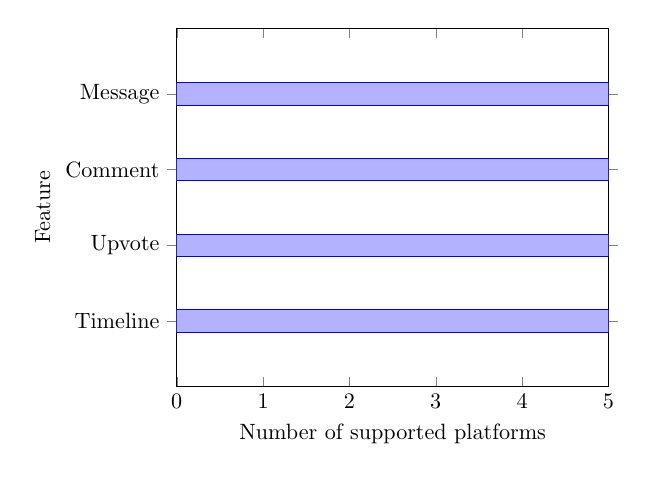
\begin{tikzpicture}[scale=0.8]
        \begin{axis}[
                enlarge y limits=0.29,
                xbar,
                xmin = 0, xmax = 5,
                symbolic y coords = {Timeline, Upvote, Comment, Message},
                xlabel={Number of supported platforms},
                ylabel={Feature}
            ]
            \addplot coordinates {
                    (5,Timeline)
                    (5,Upvote)
                    (5,Comment)
                    (5,Message)
                };
        \end{axis}
    \end{tikzpicture}
    \caption{Market analysis features}
    \label{fig:market-analysis}
\end{figure}

At first glance, \autoref{fig:market-analysis} shows that all selected platforms offer the same core functionalities.
All content is also shown on a timeline.
What is much more interesting here is how this timeline is displayed and how to configure it.
It was previously discussed that infinite scroll must be interrupted in some way.
Instagram has taken preventive measures for this.
When users scroll down the timeline, a banner that reads "Post You've already seen" will inform them that there is no more recent information from this point on.\\

Reddit, on the other hand, offers the most versatile way to configure the timeline.
There it is possible to sort the content according to different criteria.
Best shows posts with the best upvote/downvote ratio. Hot shows the posts that have currently been most upvoted and commented on.
Top generally shows the most upvotes regardless of downvotes.
The sorting by top can then continue to be sorted into specific time periods such as top posts of all time or last week.\\

All platforms except Reddit do without downvotes. Facebook and LinkedIn, on the other hand, even have more than one way to respond to content.
This can also be a useful feature, because a Like on an action in which several people died can be misinterpreted.
Instead, Facebook's sad response might be a better response.
However, more ways to react also potentially provide more ways to be misinterpreted or trolled with.
For this reason UK4You will only have a single reaction.\\

ResearchGate offers the last interesting feature regarding timelines.
Posts are given a label there, which should explain why this post is being suggested.
This seems to be an interesting to make the AI behind these posts explainable.
Many more important points and decisions were found in the market analysis.
However, this is not done here in order to avoid double mentions in the different sections.\\

\subsection{Personas}
A user persona is a model that represents fictitious users\cite[p. 123]{cooper-alan}. 
This model essentially includes both sociodemographic and psychographic characteristics.
The goal of personas is to simulate real user behavior and to adapt the software to the users.
Personas are in contrast to the abstract concept of a user because they are concrete fictional people.
Another important property of personas is that they are chosen stereotypically.
This gives the fictional characters more credibility\cite[p.127]{cooper-alan}.\\

As it turned out earlier, there are two main use cases for the platform.
An academic and a professional use case.
The persona Stefan (see \autoref{fig:persona-one}) represents the professional and Maria (see \autoref{fig:persona-two}) the academic user.
Contrary to the previous statement regarding stereotypes, Maria was given the more analytical view.
This is because there can always be situations where stereotypical expectations cannot be met.
For this reason, a small random factor should also be included in the personas.

\subsection{Scenarios}
\textcolor{red}{TODO explain scenarios}

\subsection{Scenario - Stefan}
Stefan is in a café right now.
Today he travels alone and without his usual friends.
He wants to beautify his profile on UK4You with newly learned skills so that potential employers are aware of him and his skills.
Stefan pulls out his phone and starts editing his profile page.
He has recently learned the Python programming language and feels comfortable with it.
For this reason, he enters Python as a skill under the Skills category.
However, he thinks that it might also make sense to register his participation in the university's coding club there.
So he enters this as well.
Suddenly Stefan receives a notification.
He is curious and clicks the notification.
Max1337 wrote a comment to Stefan under his skill Python: "As if you know Python what nonsense".
The automatic filter system has put the comment on-hold, which is why it is not yet visible to everyone.
Stefan thinks that this comment shouldn't visible and simply removes it.
After he removed the comment he opens the job page of the UK4You platform and looks at the different employers.
Several suggestions are already made there based on Stefan's skills.
However, he has the option to change this filter and adjust his own filter options.
With one click he sends several applications to different companies.
After doing that, he packs his cell phone back to enjoy his coffee.

\subsection{Scenario - Maria}
Maria is currently going through her daily social media routine.
She has decided to check the most important information once a day.
She just finished checking out the posts on Mastodon, a decentralized alternative to Twitter.
Maria would now like to scroll through UK4You to see the current academic work at her university.
On the timeline, she sees all the posts from all the academics she follows.
She follows current research so closely because she is interested in participating.
Fortunately, she sees a post where a professor calls for participation in a research project.
She wants to find out more and clicks on the professor's profile.
She sees that the professor has many publications and that they also represent topics in her field of interest.
For this reason, Maria decides to contact the professor.
With the help of a button, she can express her interest in the research work.

